\begin{flushright} {\tiny {\color{gray} basis\_p3\_2D.tex}} \end{flushright}
%~~~~~~~~~~~~~~~~~~~~~~~~~~~~~~~~~~~~~~~~~~~~~~~~~~~~~~~~~~~~~~~~~~~~~~~~~~~~~~~~~~~~~~~~~~~~~~~~~~

This finite element space consists of continuous piecewise cubic functions.
The functionals in a mesh cell are defined to be the values in the vertices ($d+1=2+1=3$ values), 
two values on each edge (dividing the edge in three parts of equal length) (3*2 values), 
and the value in the barycenter of the cell. 
It is implemented in \stone~120.
See also python code in {\tt images/basis\_P3} which I wrote to test these basis functions.


\begin{flushright} {\tiny {\color{gray} (tikz\_P3.tex)}} \end{flushright}
%~~~~~~~~~~~~~~~~~~~~~~~~~~~~~~~~~~~~~~~~~~~~~~~~~~~~~~~~~~~~~~~~~~~~~~~~~~~~~~~~~~~~~~~~~~~~~~~~~~

\begin{center}
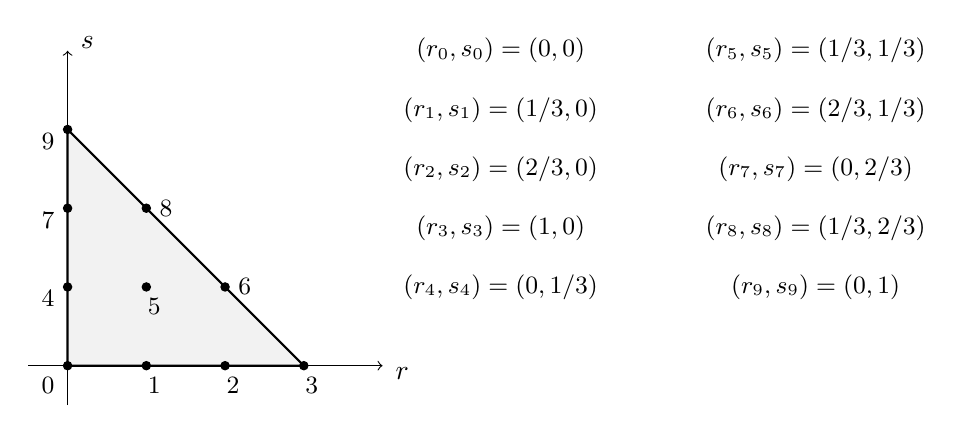
\begin{tikzpicture}
%\draw[step=0.5cm,gray,very thin] (0,0) grid (13,6); 
\draw[fill=gray!10,gray!10] (0.5,0.5)--(3.5,0.5)--(0.5,3.5)--cycle;
\draw[thick] (0.5,0.5)--(3.5,0.5)--(0.5,3.5)--cycle;
\draw [->] (0,0.5) -- (4.5,0.5);
\draw [->] (0.5,0) -- (0.5,4.5);
\node[] at (4.75,0.4) {$r$};
\node[] at (0.75,4.6) {$s$};
\draw[black,fill=black] (0.5,0.5)   circle (1.5pt);
\draw[black,fill=black] (1.5,0.5)   circle (1.5pt);
\draw[black,fill=black] (2.5,0.5)   circle (1.5pt);
\draw[black,fill=black] (3.5,0.5)   circle (1.5pt);
\draw[black,fill=black] (0.5,1.5)   circle (1.5pt);
\draw[black,fill=black] (1.5,1.5)   circle (1.5pt);
\draw[black,fill=black] (2.5,1.5)   circle (1.5pt);
\draw[black,fill=black] (0.5,2.5)   circle (1.5pt);
\draw[black,fill=black] (1.5,2.5)   circle (1.5pt);
\draw[black,fill=black] (0.5,3.5)   circle (1.5pt);

\node[] at (0.25,0.25) {\small $0$};
\node[] at (1.6,0.25)  {\small $1$};
\node[] at (2.6,0.25)  {\small $2$};
\node[] at (3.6,0.25)  {\small $3$};
\node[] at (0.25,1.35) {\small $4$};
\node[] at (1.6,1.25)  {\small $5$};
\node[] at (2.75,1.5)  {\small $6$};
\node[] at (0.25,2.35) {\small $7$};
\node[] at (1.75,2.5)  {\small $8$};
\node[] at (0.25,3.35)  {\small $9$};

\node[] at (6,4.5)  {\small $(r_0,s_0)=(0,0)$};
\node[] at (6,3.75) {\small $(r_1,s_1)=(1/3,0)$};
\node[] at (6,3)    {\small $(r_2,s_2)=(2/3,0)$};
\node[] at (6,2.25) {\small $(r_3,s_3)=(1,0)$};
\node[] at (6,1.5)  {\small $(r_4,s_4)=(0,1/3)$};

\node[] at (10,4.5)  {\small $(r_5,s_5)=(1/3,1/3)$};
\node[] at (10,3.75) {\small $(r_6,s_6)=(2/3,1/3)$};
\node[] at (10,3)    {\small $(r_7,s_7)=(0,2/3)$};
\node[] at (10,2.25) {\small $(r_8,s_8)=(1/3,2/3)$};
\node[] at (10,1.5)  {\small $(r_9,s_9)=(0,1)$};


\end{tikzpicture}
\end{center}



The basis polynomial is in this case
\[
f(r,s) = c_0 + c_1 r+ c_2 s + c_3r^2 + c_4 rs + c_5 s^2
+c_6 r^3 + c_7 r^2s + c_8 rs^2 + c_9 s^3
\]
with the requirement that it should be such that $f(r_i,s_i)=f_i$ at the 10 nodes:
\begin{eqnarray}
f_0 = f(r_0,s_0) &=& c_0 \nn\\
f_1 = f(r_1,s_1) &=& c_0 + c_1 + \frac19 c_3 + \frac{1}{27} c_6 \nn\\
f_2 = f(r_2,s_2) &=& c_0 + \frac23 c_1 + \frac{4}{9} c_3 + \frac{8}{27} c_6\nn\\
f_3 = f(r_3,s_3) &=& c_0 + c_1 + c_3 + c_6 \nn\\
f_4 = f(r_4,s_4) &=& c_0 + \frac13 c_2   + \frac19 c_5 + \frac{1}{27} c_9 \nn\\
f_5 = f(r_5,s_5) &=& c_0 + \frac13 c_1 + \frac13 c_2 + \frac19 c_3 
+ \frac19 c_4  + \frac19 c_5 + \frac{1}{27}c_6 r^3 + \frac{1}{27}c_7 + \frac{1}{27}c_8 + \frac{1}{27} c_9 \nn\\
f_6 = f(r_6,s_6) &=& c_0 + \frac23 c_1 + \frac13 c_2  
+ \frac49 c_3+ \frac29 c_4 + \frac19 c_5 + \frac{8}{27}c_6 +\frac{4}{27} c_7 +\frac{2}{27} c_8 +\frac19 c_9 \nn\\
f_7 = f(r_7,s_7) &=& c_0 + \frac23 c_2  + \frac49c_5 + \frac{8}{27}c_9 \nn\\
f_8 = f(r_8,s_8) &=& c_0 + \frac13c_1 + \frac23 c_2 + \frac19 c_3
+ \frac29 c_4  + \frac49 c_5 
+ \frac{1}{27}c_6  + \frac{2}{27}c_7  + \frac{4}{27}c_8 + \frac{8}{27}c_9 s^3 \nn\\
f_9 = f(r_9,s_9) &=& c_0 + c_2 + c_5 + c_9 \nn 
\end{eqnarray}
or,
\[
\left(
\begin{array}{cccccccccc}
1 & 0& 0&0&0&0&0&0&0&0 \\
1 & \frac13 & 0 & \frac19 &0 &0 & \frac{1}{27} & 0 & 0 & 0 \\
1 & \frac23 & 0 & \frac49 & 0 & 0 & \frac{8}{27} &0 &0 &0   \\
1 & 1 & 0 & 1 &0 & 0 &1 &0 &0 &0    \\
1 & 0 & \frac13 & 0 & 0 & \frac19 & 0& 0& 0 & \frac{1}{27}\\
1 & \frac13 & \frac13 & \frac19 & \frac19 & \frac19 & \frac{1}{27} & \frac{1}{27} & \frac{1}{27} & \frac{1}{27}    \\
1 & \frac23 & \frac13 & \frac49 & \frac29 & \frac19 
& \frac{8}{27}  & \frac{4}{27}  & \frac{2}{27}  & \frac{1}{27}    \\
1 & 0 & \frac23 & 0 & 0 & \frac49 & 0& 0& 0& \frac{8}{27}  \\
1 & \frac13 & \frac23 & \frac19 & \frac29 & \frac49 & \frac{1}{27} & \frac{2}{27} & \frac{4}{27} & \frac{8}{27}    \\
1 & 0 & 1 & 0 & 0 &1 & 0 & 0 & 0 & 1   
\end{array}
\right)
\cdot
\left(
\begin{array}{c}
c_0 \\ c_1 \\ c_2 \\ c_3 \\ c_4 \\ c_5 \\ c_6 \\ c_7 \\ c_8 \\ c_9
\end{array}
\right)
=
\left(
\begin{array}{c}
f_0 \\ f_1 \\ f_2 \\ f_3 \\ f_4 \\ f_5 \\ f_6 \\ f_7 \\ f_8 \\ f_9
\end{array}
\right)
\]
or, 
\[
\frac{1}{27}
\left(
\begin{array}{cccccccccc}
27 & 0& 0&0&0&0&0&0&0&0 \\
27 & 9 & 0 & 3 &0 &0 & 1 & 0 & 0 & 0 \\
27 & 18 & 0 & 12 & 0 & 0 & 8 &0 &0 &0   \\
27 & 27 & 0 & 27 &0 & 0 &27 &0 &0 &0    \\
27 & 0 & 9 & 0 & 0 & 3 & 0& 0& 0 & 1\\
27 & 9 & 9 & 3 & 3 & 3 & 1 & 1 & 1 & 1    \\
27 & 18 & 9 & 12 & 6 & 3 & 8  & 4  & 2  & 1    \\
27 & 0 & 18 & 0 & 0 & 12 & 0& 0& 0& 8  \\
27 & 9 & 18 & 3 & 6 & 12 & 1 & 2 & 4 & 8\\
27 & 0 & 27 & 0 & 0 &27 & 0 & 0 & 0 & 27  
\end{array}
\right)
\cdot
\left(
\begin{array}{c}
c_0 \\ c_1 \\ c_2 \\ c_3 \\ c_4 \\ c_5 \\ c_6 \\ c_7 \\ c_8 \\ c_9
\end{array}
\right)
=
\left(
\begin{array}{c}
f_0 \\ f_1 \\ f_2 \\ f_3 \\ f_4 \\ f_5 \\ f_6 \\ f_7 \\ f_8 \\ f_9
\end{array}
\right)
\]
The inverse of the matrix is 
\[
\frac12
\left(
\begin{array}{cccccccccc}
2 &0 &0 &0 &0 &0 &0 &0 &0 &0\\
-11 & 18 & -9 & 2 &0 &0 &0 &0 &0 & 0 \\
-11 & 0 & 0 & 0 & 18 & 0 & 0 & -9 & 0 & 2 \\
18 & -45 & 36 &-9 &  0& 0& 0& 0& 0& 0 \\
36 &-45 & 9 & 0 &  -45 & 54 &-9 & 9 &  -9 & 0\\
18 &0& 0& 0 & -45& 0 &0 & 36& 0 &-9 \\
-9 & 27 &-27 & 9 &  0 & 0 & 0 & 0  &  0 & 0\\
-27 & 54& -27& 0& 27 &-54 & 27 &0 &0 &0 \\
-27 & 27 &0 &0 &54& -54 &0 &-27  &  27 &0 \\
-9 &0 &0 &0 &27 &0& 0 &-27 &0&  9
\end{array}
\right)
\]
so that the solution of the system ${\bm A}\cdot \vec{c}=\vec{f}$ is
$\vec{c} = {\bm A}^{-1}\cdot \vec{f}$, or:
\begin{eqnarray}
c_0 &=& 1   \nn\\
c_1 &=& \frac12 (-11 f_0 + 18 f_1 -9 f_2 + 2f_3 ) \nn\\
c_2 &=& \frac12 (-11f_0 + 18f_4 -9 f_7 + 2f_9) \nn\\
c_3 &=& \text{etc ...}
\end{eqnarray}
which we insert in 
\[
f(r,s) = c_0 + c_1 r+ c_2 s + c_3r^2 + c_4 rs + c_5 s^2
+c_6 r^3 + c_7 r^2s + c_8 rs^2 + c_9 s^3
\]
and we then obtain
\begin{eqnarray}
f(r,s) 
&=&\frac12\left(2-11r-11s+18r^2+36rs+18s^2-9r^3-27r^2s-27rs^2-9s^3 \right) f_0 \nn\\
&+&\frac12\left(18r-45r^2-45rs +27r^3 +54r^2s+27rs^2\right) f_1\nn\\
&+&\frac12\left( -9r+36r^2+9rs -27r^3 -27r^2s \right) f_2\nn\\
&+&\frac12\left( 2r-9r^2+9r^3 \right) f_3\nn\\
&+&\frac12\left( 18s -45rs-45s^2+27r^2s+54rs^2+27s^3\right) f_4\nn\\
&+&\frac12\left( 54rs-54r^2s-54rs^2  \right) f_5\nn\\
&+&\frac12\left( -9rs+27r^2s  \right) f_6\nn\\
&+&\frac12\left( -9s+9rs+36s^2-27rs^2-27s^3  \right) f_7\nn\\
&+&\frac12\left( -9rs+27rs^2  \right) f_8\nn\\
&+&\frac12\left( 2s-9s^2+9s^3  \right) f_9 \nn \\
&=& \sum_{i=0}^9 \bN_i(r,s) f_i \nn
\end{eqnarray}
with
\begin{mdframed}[backgroundcolor=blue!5]
\begin{eqnarray}
\bN_0(r,s) &=& \frac12\left(2-11r-11s+18r^2+36rs+18s^2-9r^3-27r^2s-27rs^2-9s^3 \right)   \nn\\
\bN_1(r,s)&=& \frac12\left(18r-45r^2-45rs +27r^3 +54r^2s+27rs^2\right)   \nn\\
\bN_2(r,s)&=& \frac12\left( -9r+36r^2+9rs -27r^3 -27r^2s \right)   \nn\\
\bN_3(r,s)&=& \frac12\left( 2r-9r^2+9r^3 \right)   \nn\\
\bN_4(r,s)&=& \frac12\left( 18s -45rs-45s^2+27r^2s+54rs^2+27s^3\right) \nn\\
\bN_5(r,s)&=& \frac12\left( 54rs-54r^2s-54rs^2  \right)   \nn\\
\bN_6(r,s)&=& \frac12\left( -9rs+27r^2s  \right)   \nn\\
\bN_7(r,s)&=& \frac12\left( -9s+9rs+36s^2-27rs^2-27s^3\right)\nn\\
\bN_8(r,s)&=& \frac12\left( -9rs+27rs^2  \right)   \nn\\
\bN_9(r,s)&=& \frac12\left( 2s-9s^2+9s^3  \right)   
\end{eqnarray}
\end{mdframed}
and 
\begin{eqnarray}
\frac{\partial\bN_0}{\partial r} (r,s) &=& \frac12(-11+36r+36s-27r^2-54rs-27s^2)   \nn\\
\frac{\partial\bN_1}{\partial r} (r,s) &=& \frac12(18-90r-45s+81r^2+108rs+27s^2)   \nn\\
\frac{\partial\bN_2}{\partial r} (r,s) &=& \frac12(-9+72r+9s-81r^2-54rs)   \nn\\
\frac{\partial\bN_3}{\partial r} (r,s) &=& \frac12(2-18r+27r^2)   \nn\\
\frac{\partial\bN_4}{\partial r} (r,s) &=& \frac12(-45s+54rs+54s^2)   \nn\\
\frac{\partial\bN_5}{\partial r} (r,s) &=& \frac12(54s-108rs-54s^2) \nn\\
\frac{\partial\bN_6}{\partial r} (r,s) &=& \frac12(-9s+54rs) \nn\\
\frac{\partial\bN_7}{\partial r} (r,s) &=& \frac12(9s-27s^2) \nn\\
\frac{\partial\bN_8}{\partial r} (r,s) &=& \frac12(-9s+27s^2)\nn\\
\frac{\partial\bN_9}{\partial r} (r,s) &=&  0  \nn
\end{eqnarray}

\begin{eqnarray}
\frac{\partial\bN_0}{\partial s} (r,s) &=& \frac12(-11+36r+36s-27r^2-54rs-27s^2)   \nn\\
\frac{\partial\bN_1}{\partial s} (r,s) &=& \frac12(-45r+54r^2+54rs)   \nn\\
\frac{\partial\bN_2}{\partial s} (r,s) &=& \frac12(9r-27r^2)   \nn\\
\frac{\partial\bN_3}{\partial s} (r,s) &=& 0   \nn\\
\frac{\partial\bN_4}{\partial s} (r,s) &=& \frac12(18-45r-90s+27r^2+108rs+81s^2)   \nn\\
\frac{\partial\bN_5}{\partial s} (r,s) &=& \frac12(54r-54r^2-108rs)   \nn\\
\frac{\partial\bN_6}{\partial s} (r,s) &=& \frac12(-9r+27r^2)   \nn\\
\frac{\partial\bN_7}{\partial s} (r,s) &=& \frac12(-9+9r+72s-54rs-81s^2)   \nn\\
\frac{\partial\bN_8}{\partial s} (r,s) &=& \frac12(-9r+54rs)   \nn\\
\frac{\partial\bN_9}{\partial s} (r,s) &=& \frac12(2-18s+27s^2)   \nn
\end{eqnarray}


In barycentric coordinates the basis functions are:
\begin{itemize}
\item on the nodes: $\frac12\lambda_i (3\lambda_i-1)(3\lambda_i-2) $
\item on the edges: $\frac92 \lambda_i \lambda_j(3\lambda_i-1)$
\item in the middle: $27\lambda_i\lambda_j\lambda_k$
\end{itemize}

Probably found in John's book - need to check that!

















